\chapter{Perspectives}
\label{chapter_perspectives}
The different perspectives that can display a news article will be presented and following in this chapter is a more thorough examination of how the different perspectives are related, how one perspective translates to another, the transition between them, and which perspectives fits which purposes.


\section{The Different Perspectives}
\label{perspectives_presentation}
There are a lot of different ways that news can be presented, considering how much information from a news article that are shown, how it is shown graphically, what the information shown means in different contexts etc. Following are description of the perspectives that are most used in different news applications and the applications referred to in this section are examined and presented in section \ref{commercial_news_applications}.

\subsubsection{Full Article}
A full article perspective, as the name implies, is perspective that normally holds all the information available for that particular news story. The most important information in this perspective is the full article text, as this is the information that most often is lacking in the other perspectives. Figure \ref{full_article_prismatic} shows an example of a full article perspective.

\begin{figure}[!htbp]
\centering
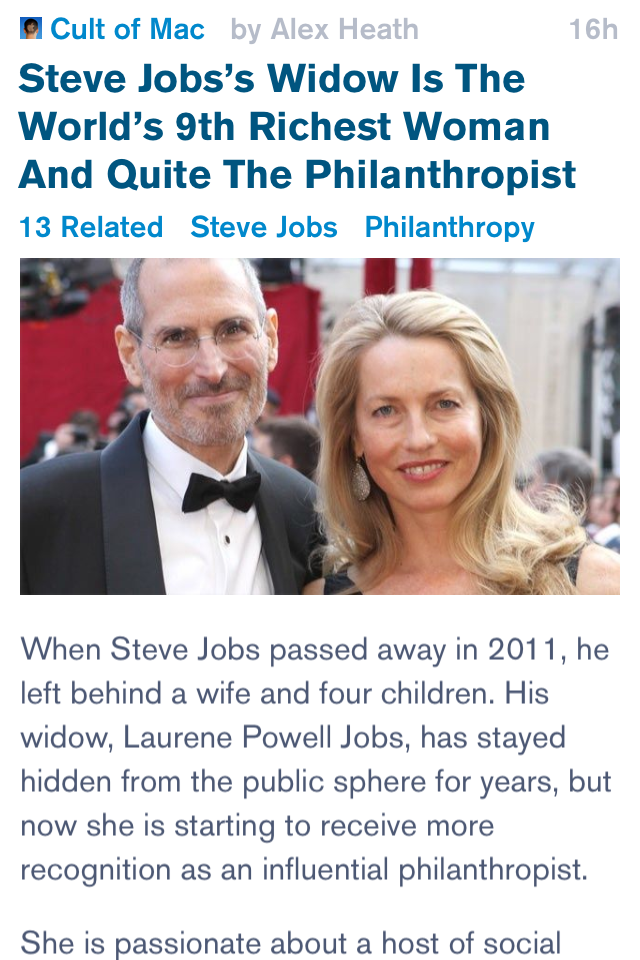
\includegraphics[width=50mm]{GFX/perspectives/fullArticleViewPrismatic.png}
\caption{A screenshot from Prismatic showing an example of a full article perspective.}
\label{full_article_prismatic}
\end{figure}

\subsubsection{RSS}
An RSS perspective is a perspective showing just some of the information from an article to give the user a quick overview of what the news article concerns. The name stems from the RSS feed technology which has a certain set of information like title, lead-text, when the article was published, and sometimes an image. The RSS view may have other information as well, but the ones mentioned are the most common. Figure \ref{rss_feedly} shows an example of how an RSS perspective may be presented.

\begin{figure}[!htbp]
\centering
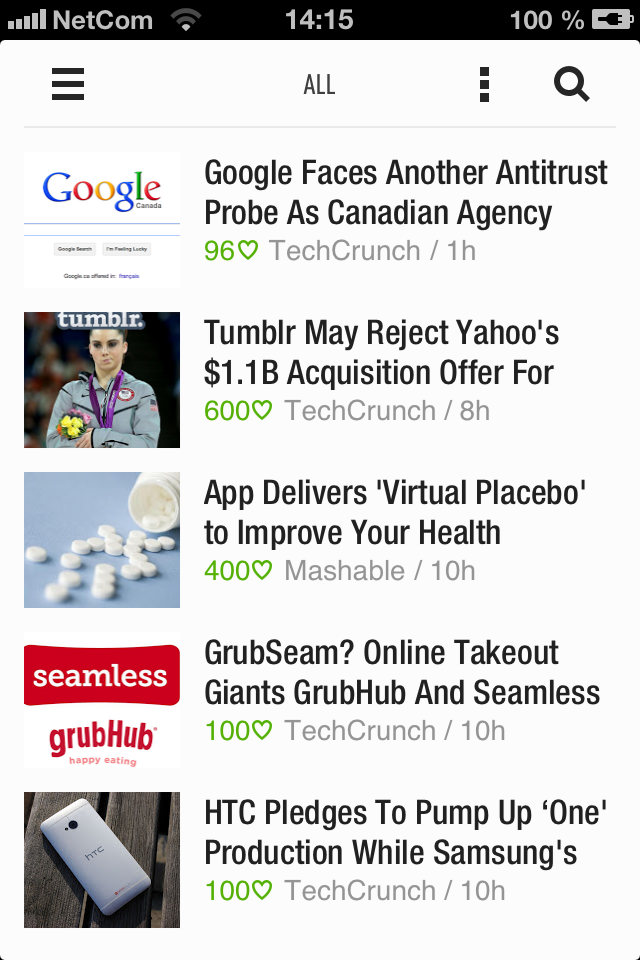
\includegraphics[width=50mm]{GFX/perspectives/rssViewFeedly.png}
\caption{A screenshot from Feedly showing an example of an RSS perspective.}
\label{rss_feedly}
\end{figure}

\subsubsection{Entity}
An entity perspective is a perspective showing a set of keywords extracted from a news article by the use of a keyword extracting algorithm or other NLP technologies. Figure \ref{entity_news_cloud} shows an example of how an entity perspective can be displayed to the user. In this application if a keyword is selected, all the other keywords that are connected to this keyword is highlighted. The articles these keywords are extracted from are shown in a view on the right-hand side as links that will take the user to the corresponding article if clicked.

\begin{figure}[!htbp]
\centering
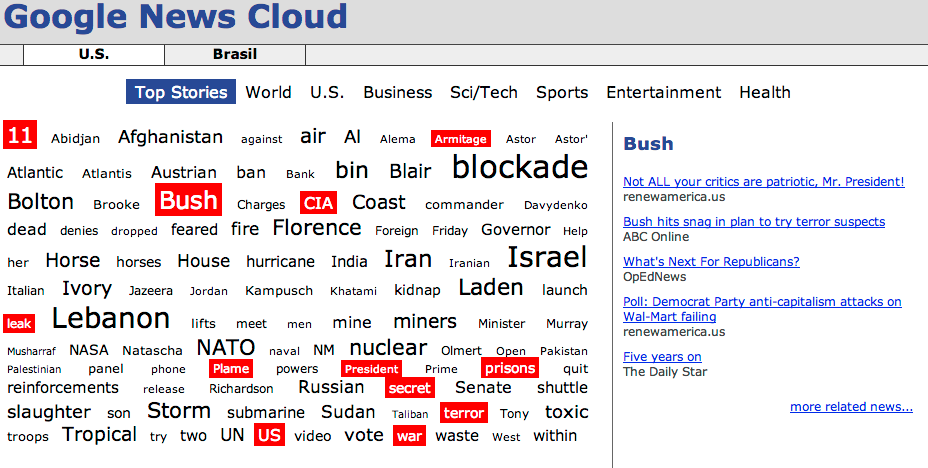
\includegraphics[width=140mm]{GFX/perspectives/entityViewNewsCloud.png}
\caption{A screenshot from NewsCloud showing an example of an entity perspective.}
\label{entity_news_cloud}
\end{figure}

\subsubsection{Event}
An event perspective is a perspective that displays certain events that occurred by analyzing news articles and extracting those events by using NLP or other text-analyzing techniques. Figure \ref{event_wavii} shows three events extracted from different news articles. The first shows that two celebrities broke up, the second shows that a theatrical trailer was released by a movie publisher and the third shows that a software company released a new application for the iOS platform.

\begin{figure}[!htbp]
\centering
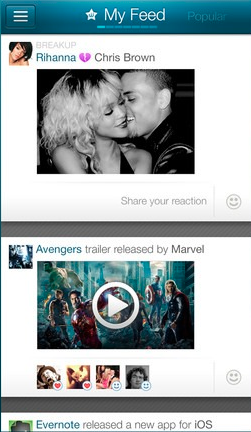
\includegraphics[width=50mm]{GFX/perspectives/eventViewWavii.png}
\caption{A screenshot from Wavii showing an example of an event perspective.}
\label{event_wavii}
\end{figure}

\subsubsection{Web}
The web perspective is quite similar to the full article perspective and usually includes the same amount of information. The main difference is that the web perspective is the news article shown at the publisher's website through an application by the use of a web browser inside a third party application. This is a widely used perspective as a third party application cannot normally show a full news article from another publisher without an agreement with the publisher itself. Showing a full article without a contract with the publisher is most likely a copyright infringement. Figure \ref{web_flipboard} shows an example of how a web perspective may be presented.

\begin{figure}[!htbp]
\centering
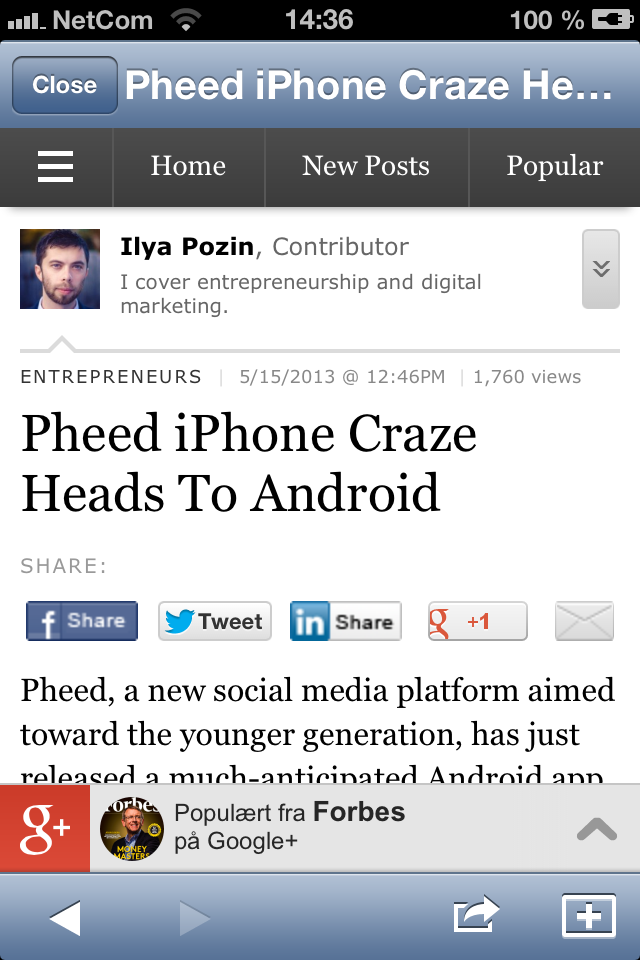
\includegraphics[width=50mm]{GFX/perspectives/webViewFlipboard.png}
\caption{A screenshot from Flipboard showing an example of a web perspective.}
\label{web_flipboard}
\end{figure}

\subsubsection{Summary}
The summary perspective is a perspective that shows a summary text of the full article text, where this text is created by the use of NLP technologies, like the Summly application, or hand crafted by real editors, like the Circa application. Figure \ref{summary_summly} shows a screenshot of the Summly application presenting a summary perspective.

\begin{figure}[!htbp]
\centering
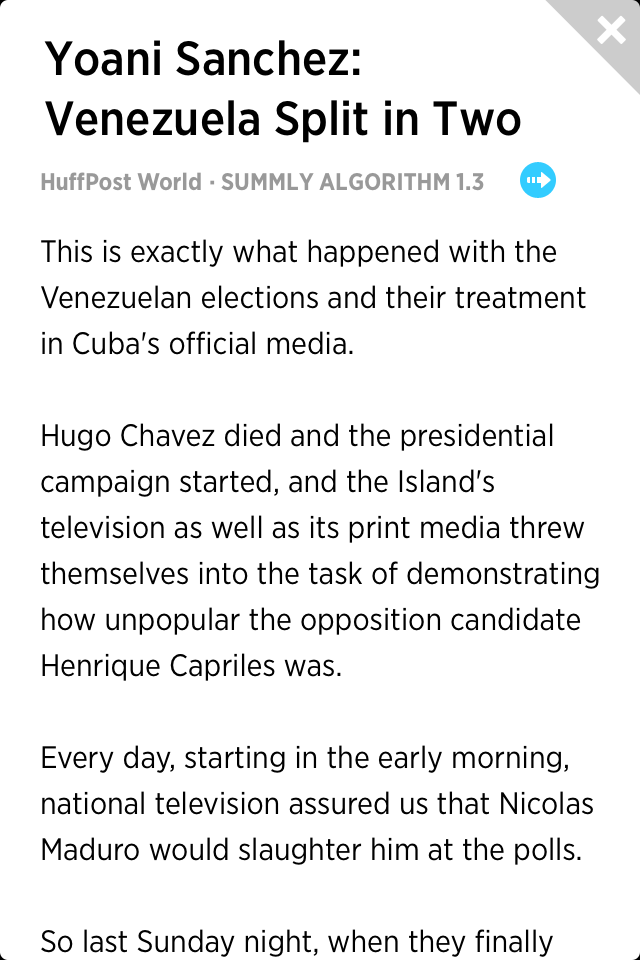
\includegraphics[width=50mm]{GFX/perspectives/summaryViewSummly.png}
\caption{A screenshot from Summly showing an example of a summary perspective.}
\label{summary_summly}
\end{figure}

\subsubsection{Map}
The map perspective is a perspective that shows where in the world a news story concerns by the use of a map view. Figure \ref{map_circa} shows a news story residing in Lisbon, Portugal in the Circa application.

\begin{figure}[!htbp]
\centering
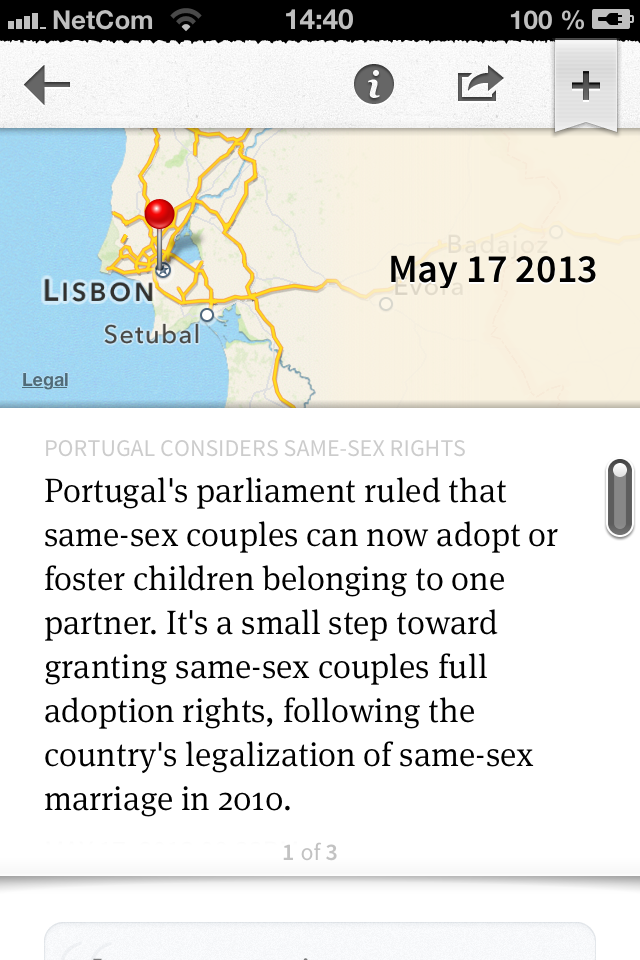
\includegraphics[width=50mm]{GFX/perspectives/mapViewCirca.png}
\caption{A screenshot from Circa showing an example of a map perspective.}
\label{map_circa}
\end{figure}

\section{Relations}
A perspective can present all the information available from a news article or just a subset of the information, depending on which purpose the perspective has and what type of information the perspective is trying to convey. Following is an explanation of how the different perspectives are related.

\subsubsection{Full Article Perspective and Web Perspective}
The full article perspective and the web perspective are the two perspectives that holds the most information and are most related. The main difference between the two is that the full article perspectives presents its information in a native way, following the UI design that goes with rest of the application, while the web perspective is presented as a web page in a web browser wrapper inside the native application. The full article perspective is designed by the creator of the native application, while the web perspective usually is designed by the content publisher itself as a responsive web page\footnote{A responsive web page is web page that adapts to the screen size and resolution of the device opening the web page.}. If a native app developer wants to show all information available from a news article, it usually has to be done via a web perspective to avoid copyright infringement. The developer can present it as a full article perspective if the app developer has some kind of agreement with content publisher who has the copyright, or the app developer is the content publisher itself.

\subsubsection{RSS Perspective}
All the other perspectives presents information that can somehow be derived from the full article perspective or the web perspective. The RSS perspective normally holds the information that are available from an RSS feed, hence the name, which is information that usually are available and free to use from the content publishers itself, as long as it links to the web perspective of the same article.

\subsubsection{Entity Perspective}
The entity perspective holds information in terms of keywords. Normally these keywords are not available from any content supplier, but has been processed from the news article's title, lead text, and full article text, by the use of some sort of keyword extraction algorithm or other NLP technologies. For the best result the event perspective is derived from the full article perspective or web perspective to be able to process all of the information available, but it can also be derived from the RSS perspective, as the title and lead text alone often holds important keywords that are sufficient to understand what the articles comprises.

\subsubsection{Event Perspective}
Similar to the entity perspective, the event perspective holds information that are derived and processed from the full article perspective or the web perspective. To extract the information shown in the event perspective, advanced NLP technology needs to be applied and a deeper understanding of the article needs to be established. Deriving information from the RSS perspective is most likely not sufficient to overcome this. An event may be extracted from the RSS perspective, but titles and lead texts alone may be misleading or not convey fully what the full story text tries to communicate.

\subsubsection{Summary Perspective}
NLP is a fairly important domain when processing news articles and extracting useful information, and the summary perspective is another example of just this. As the name implies, the summary perspective most often shows a summary of the full article text derived from the full article perspective or web perspective. The summaries can be created by the use of NLP, like the Summly application, or by real editors like the Circa application. The summary perspective are not limited to a text summary, it can also hold information from the entity perspective and the event perspective as these also are a form of summaries or compressed information from the full article perspective or web perspective.

\subsubsection{Map Perspective}
To be able to show on a map where news articles resides, the information from the full article perspective or web perspective needs to be thoroughly processed and analyzed, and again NLP is an important part of this. Places can be extracted from the title, lead text or the full article text, but this information is not sufficient to say where an article's content concerns. There are several challenges to overcome to accomplish an accurate map perspective. 

The name of a place without knowing the coordinates of the place, can point to several places throughout the globe. For instance, Heimdal is a place near Trondheim, Norway, but is also a place in North Dakota, USA. To be able to pick the right one, a deeper understanding of the article is necessary. 

Also an article can mention several places in the full article text, without all of these places necessarily concerns the article itself. For instance, the article can state "The rock and roll band Aerosmith from Boston, Massachusetts is playing the O2 arena in London next week, with support from the electronica band Röyksopp from Tromsø, Norway". In this example London would be the place the article concerns, and Boston and Tromsø are places that would be misleading to pin to a map with same significance as London.


\section{Purpose of and Flow Between Perspectives}
The different perspectives serves different purposes, and have various areas of usage. Following are a description of the perspectives' main functions and where they convey their information to the fullest, ordered after when they are most likely to appear to the user. The more information the perspective can hold the farther down in the navigation hierarchy they are likely to be.


\subsubsection{RSS Perspective}
The RSS perspective often serves as an entry point to a news article and its purpose is to give a quick overview of the content of the article and/or to trigger a curiosity at the user's end to make them wanting to read more. The information in the RSS perspective are often authored by a journalist from the content publisher to achieve exactly this purpose, to drive more traffic to the content publisher's web page, which again will give the content publisher more advertising revenue. With this in mind the RSS perspective is on a thin line between supplying enough information to give the user an understanding of what the topic and main content of the article is, but at the same time create enough curiosity to make the user wanting to read more.

\subsubsection{Summary Perspective}
The summary perspective is located somewhere in between the RSS perspective and the full article perspective or web perspective in the navigation hierarchy. For the users that want a little bit more information than what the RSS perspective can provide, but less than the full article perspective has to offer, it can serve as a replacement for both. It can work well as an entry point to an article and at the same time provide enough information to the user to make it satisfied with the information it has gained from the summary text. 

It can also serve as an additional level in the navigation hierarchy, between the RSS perspective and the full article perspective or web perspective, to give the user smaller steps between the perspectives and the amount of information presented.

\subsubsection{Event Perspective}
The event perspective shows important events extracted from the news article and is in a way a short summary consisting of the most important happenings in an article. For users browsing through many articles, this is a simple and efficient way to get the most important parts of an article. For these users an event perspective can work as an entry point to an article and replace the normally used RSS perspective. For some users the event perspective can also work as a replacement of the summary perspective, given that the events covers the essential content in the article. Similar to the summary perspective, the event perspective also can serve as an additional level in the navigation hierarchy to supply the user with some extra information in addition to the RSS perspective before deciding to navigate to the full article perspective.

\subsubsection{Entity Perspective}
The entity perspective can serve two main purposes. If presented as a supplemental perspective to the full article perspective or web perspective in the same level in the navigation hierarchy, it can serve as a way to find related articles and topics based on a news article. If, for instance, the entities in an entity view are "war, Bush, Al-Qaeda, Middle East, Iraq", these keywords can work as buttons to display a cluster of news about one of those keywords, or they can be added to the user profile as an interesting topic to be included when recommending news articles.

On the other hand, the entity view can serve as a way of getting a quick overview of what the main topics of an article are and then decide to go further into the navigation hierarchy to read more about it. Considering the example given over, a user can easily decide if this is a topic worth reading more about, or skip through. With this approach the entity perspective could replace the RSS perspective, and even the summary or event perspective for some users.


\subsubsection{Full Article Perspective}
The full article perspective has all the news article's information available, and are usually the last level in the navigation hierarchy. It is the perspective for the most interested users, who wants to have access to all the information an article has to offer, and to be able to read the whole story. This is a perspective primarily used by applications that have legal access to all the content of a story, like the content publishers themselves or third-party developers with special agreements with the content publishers.

\subsubsection{Web Perspective}
The web perspective serves the same purpose as the full article perspective, to satisfy the most interested users. This perspective are also usually located at the end of the navigation hierarchy, normally linked to from the RSS perspective, or one of the other perspectives that can replace the RSS perspective or work as a middle layer between the RSS perspective and web perspective, like the summary, event, or entity perspective.


\subsubsection{Map Perspective}
The map perspective has two main purposes. It can work as an additional perspective to the full article perspective or web perspective to show the user on a map where an article resides, to provide the interested user even more information about the content.

It can also work as an entry point, but this can become a foul experience if not done right and then defeat its purpose. If used as an entry point, it would probably not be of much use to show a lot of articles spread out all over the world on a such small device, and have the user click every map pin to see if this could be an interesting story or not. On the other hand if the device can collect the users location and retrieve news that are nearby with coordinates that are accurate to where the news story concerns, the user can probably have a better understanding of the location, since the user is located nearby and probably knows the area better and can easier relate to the location. Then if a map pin is clicked the user can be brought further down in the navigation hierarchy.


\section{Perspectives and Their Connections in the Different Apps}
Following is a simple navigation chart showing how the different perspectives in the different applications are connected.

\subsection{Zite}

\begin{figure}[!htbp]
\centering
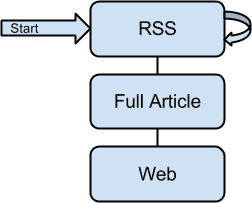
\includegraphics[width=50mm]{GFX/statecharts/Zite.png}
\caption{A simple navigation chart showing the connection between perspectives in the mobile news application Zite.}
\label{state_chart_zite}
\end{figure}

Figure \ref{state_chart_zite} shows that Zite first presents the user with the RSS perspective showing the top stories based on the user profile. Further the user can navigate from this perspective to the full article perspective by clicking one of the articles or navigate to a new RSS perspective listing articles from a topic. To move to the topic RSS perspective, the user can either search for a topic, click one the keywords that is connected to the story showing in the top stories RSS perspective, or selecting one of the topics already stored by the user. The RSS perspective can always open a new RSS perspective by clicking one of the topics associated with an article. Whenever a story is clicked in the RSS perspective, the full article perspective is shown, and from the full article perspective the user can navigate to the web perspective

\subsection{Flipboard}

\begin{figure}[!htbp]
\centering
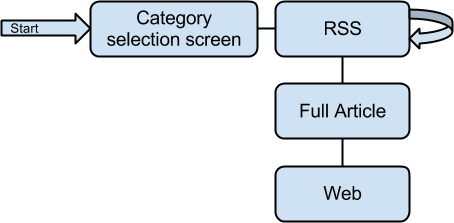
\includegraphics[width=80mm]{GFX/statecharts/Flipboard.png}
\caption{A simple navigation chart showing the connection between perspectives in the mobile news application Flipboard.}
\label{state_chart_flipboard}
\end{figure}

Figure \ref{state_chart_flipboard} shows that Flipboard greets the user with a category selection screen. From here the user can select a category that is predefined by the user or search for a topic, which in either way brings the user to the RSS perspective. From the RSS perspective the user can again search for a topic which will navigate to new RSS perspective or click an article and be presented with the full article perspective. From the full article perspective, the user can navigate to the web perspective.

\subsection{Pulse}

\begin{figure}[!htbp]
\centering
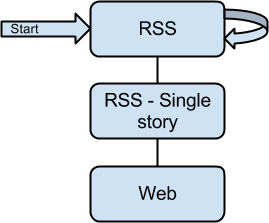
\includegraphics[width=50mm]{GFX/statecharts/Pulse.png}
\caption{A simple navigation chart showing the connection between perspectives in the mobile news application Pulse.}
\label{state_chart_pulse}
\end{figure}

Figure \ref{state_chart_pulse} shows that Pulse greets the user with the RSS perspective. This RSS perspective lists a number of RSS feeds within a certain category. The user can navigate from here to another RSS perspective listing RSS feeds from another category or search for other content and open this content in the same RSS perspective. If a story is clicked, the user is presented with another RSS perspective, but for a single article. From this single article RSS perspective, the user can navigate to the web perspective to show the whole article at the content publishers web site. 

\subsection{Summly}

\begin{figure}[!htbp]
\centering
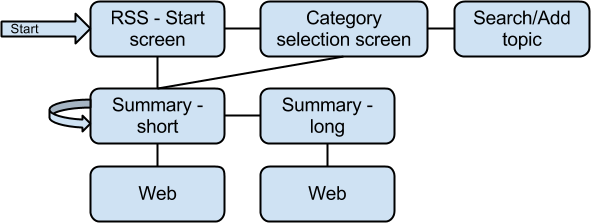
\includegraphics[width=100mm]{GFX/statecharts/Summly.png}
\caption{A simple navigation chart showing the connection between perspectives in the mobile news application Summly.}
\label{state_chart_summly}
\end{figure}

Summly starts off by presenting the user with an RSS perspective holding one trending news article, as shown in figure \ref{state_chart_summly}. From here the user can open this news article in a short summary perspective or navigate to the category selection screen. In the category selection screen the user can search for and add new topics to the category list or click a category or topic to present the short summary perspective. Once in the short summary perspective, the user can navigate between different articles in this category by performing a horizontal swipe, open a long summary perspective by double tapping the article or open the web perspective showing the whole article at the content publishers own web site. The user can also navigate to the web perspective from the long summary perspective, but not navigate between articles from here.

\subsection{News360}

\begin{figure}[!htbp]
\centering
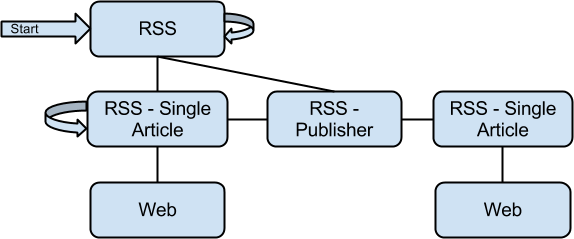
\includegraphics[width=100mm]{GFX/statecharts/News360.png}
\caption{A simple navigation chart showing the connection between perspectives in the mobile news application News360.}
\label{state_chart_news360}
\end{figure}

News360 starts by presenting the user with an RSS perspective containing the top stories based on the user profile, as shown in figure \ref{state_chart_news360}. In this perspective, the user can navigate between the stories in this category or topic by performing a horizontal swipe. From here the user can also reload the RSS perspective by selecting a different category or by searching for another topic or category. The user can navigate from this perspective to an RSS perspective showing a single article or to an RSS perspective showing a list of articles published by a single publisher by clicking on the publisher name as well. The publisher RSS perspective can open single articles from this publisher in an RSS perspective, and further open a web perspective showing the same article.

The single article RSS perspective on the left-hand side in figure \ref{state_chart_news360}, shows the article clicked in the first RSS perspective. In this perspective the user can access the web perspective showing this article at the content publishers website. The user can also choose to open other similar articles covering the same story in this perspective. The RSS perspective holding a list of a publisher's stories, can also be accessed from this perspective.

\subsection{Circa}

\begin{figure}[!htbp]
\centering
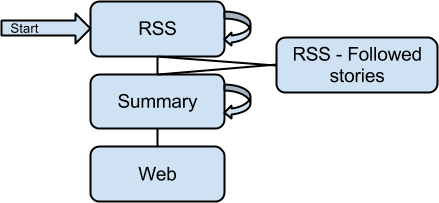
\includegraphics[width=80mm]{GFX/statecharts/Circa.png}
\caption{A simple navigation chart showing the connection between perspectives in the mobile news application Circa.}
\label{state_chart_circa}
\end{figure}

As shown in figure \ref{state_chart_circa}, the user is presented with an RSS perspective showing the top stories. The user can reload this perspective by selecting another category to show articles from. The user can also access an RSS perspective holding stories that are followed by the user from the initial RSS perspective. Further both the latter RSS perspectives links to a summary perspective. From this perspective the user can navigate to the web perspective to show the articles that the summaries are based upon, or the user can navigate to summaries of other related articles. The summary perspective can also contain a map perspective, but the map perspective does not have any interactions connected to it, it only shows where the articles concerns.

\subsection{Wavii}

\begin{figure}[!htbp]
\centering
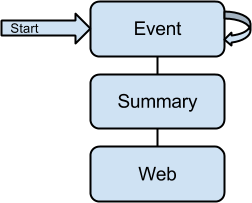
\includegraphics[width=50mm]{GFX/statecharts/Wavii.png}
\caption{A simple navigation chart showing the connection between perspectives in the mobile news application Wavii.}
\label{state_chart_wavii}
\end{figure}

Wavii presents the user with a event perspective holding a list of different events within a category or topic, as shown in figure \ref{state_chart_wavii}\footnote{The navigation chart for Wavii might not be completely accurate as the chart was based on previous notes because of the application's removal from the App Store}. The user can reload the event perspective with other topics or categories the user has chosen to follow. If an event is clicked, Wavii shows a summary of the stories that caused the event in a summary perspective. Further the user can choose to open the stories that caused the event in a web perspective.

\subsection{Prismatic}

\begin{figure}[!htbp]
\centering
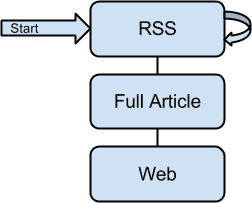
\includegraphics[width=50mm]{GFX/statecharts/Prismatic.png}
\caption{A simple navigation chart showing the connection between perspectives in the mobile news application Prismatic.}
\label{state_chart_prismatic}
\end{figure}

Prismatic greets the user with an RSS perspective holding news that are recommended for the user based on its profile, as shown in figure \ref{state_chart_prismatic}. From here the user can reload the initial RSS perspective by clicking one of the topics that are connected to an article, clicking topics that are suggested by Prismatic based on the user profile or searching for other topics. When an article is clicked it is shown in a full article perspective. From here the user can load a new RSS perspective showing related stories, stories based on topics connected to a story, or stories from a single content publisher. The story itself also contains a lot of highlighted keywords that, when pressed, opens a web perspective showing content regarding this keyword. This content can be another news story, or a page explaining a certain term etc.

\subsection{Taptu}

\begin{figure}[!htbp]
\centering
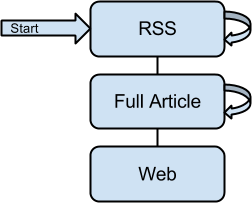
\includegraphics[width=50mm]{GFX/statecharts/Taptu.png}
\caption{A simple navigation chart showing the connection between perspectives in the mobile news application Taptu.}
\label{state_chart_taptu}
\end{figure}

As shown in figure \ref{state_chart_taptu}, Taptu greets the user with an RSS perspective that holds several lists with different categories and feeds. These lists can be modified in several ways, like merged and split, and new feeds can be added by searching or choosing some predefined feeds. When an article is clicked, the full article perspective is shown containing that article. The user can navigate between articles in this list by performing a horizontal swipe, and also open the showing article in a web perspective. The article may also contain references to other content, which is opened in a web perspective if clicked.

\subsection{Feedly}

\begin{figure}[!htbp]
\centering
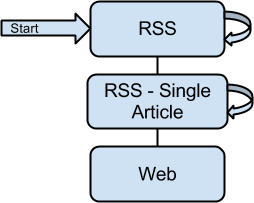
\includegraphics[width=50mm]{GFX/statecharts/Feedly.png}
\caption{A simple navigation chart showing the connection between perspectives in the mobile news application Feedly.}
\label{state_chart_feedly}
\end{figure}

Feedly starts off by presenting the user with a RSS perspective, as shown in figure \ref{state_chart_feedly}, containing a news list from all of the topics or feeds the user has stored. This RSS perspective can be reloaded, either by searching for a topic or by selecting a category or topic that the user has already stored. If an article is clicked, another RSS perspective is shown, but holding the article that was clicked. The user can navigate between the articles in the list by swiping horizontally in the single article RSS perspective and also open the article in a web perspective containing the full article at the content publisher's web site.


\subsection{Use Case}

\begin{figure}[!htbp]
\centering
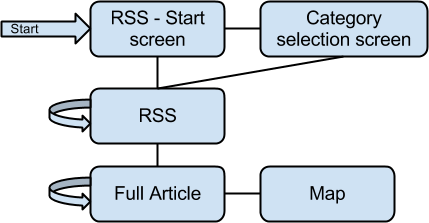
\includegraphics[width=80mm]{GFX/statecharts/UseCase.png}
\caption{A simple navigation chart showing the connection between perspectives in the use case mobile news application.}
\label{state_chart_usecase}
\end{figure}

The use case application starts off by presenting the user with an RSS perspective, as shown in figure \ref{state_chart_usecase}, consisting of the latest top story from the recommendation based on the user profile. From here the user can navigate to the category selection screen, and from the start screen or the category selection screen, the user can navigate to the RSS perspective holding articles from the top stories, the category clicked in the category selection screen or by searching for a topic in the start screen. This RSS perspective shows only one article at a time, but by performing a horizontal swipe the user can navigate between the different articles in this category. From this RSS perspective the user can navigate to the full article perspective, which also holds only one article at a time, but to access related stories the user can swipe horizontally. The map perspective, which shows where the article concerns are also accessible from the full article perspective.

\section{How the Perspectives Are Supported on the Mobile Platform}

Following is a description of how the different perspectives are supported on the mobile platform with regard to which technologies and opportunities they make use of, and how they are realized. This is, as mentioned earlier, from a iOS point of view, but applies to most other smart phones as well, as these technologies or opportunities are widely used on several mobile platforms.

To represent data, the data must be gathered and parsed in some way. News publishers most often gather and create their own data through the work of journalists. Third-party developers creating news applications often start by gathering different RSS feeds and process these further. Either way, mobile news applications need to get their data from somewhere, parse this data and represent it in some way. Raw data transferred over the Internet often is represented by XML or JSON, and parsing this data is the first step for being able to represent any of the perspectives. Some of the mobile operating systems has native support for parsing XML or JSON, and if not, there are numerous external libraries that support this that are easy accessible and free to use.

Further when the data is parsed, a way of representing the data has to be found. As all of the major mobile operating systems has native support for displaying text, images, sound and video, there just a matter of how to display it in a usable manner.

All perspectives listed in section \ref{perspectives_presentation}, except the web perspective and map perspective, normally uses parsed raw data, and can be represented as the developer wishes. Also these perspectives normally does not represent the data in any other form than text, image, video or sound, which are all natively supported.

The map perspective uses a map to pin the article's location on. It may also show some sort of text, like the title, connected to the map pin. Opening a map view inside an application is also natively supported on all the major mobile operating systems, making this, if not a trivial task, a fairly easy task.

The web perspective however, is not a perspective the developer can control much over. Opening a web page inside a mobile application is supported by the operating systems, but the layout of the content and how it is represented is controlled by the content publishers managing the web page. The native application can control the zoom level of the content and it usually has to support some sort of navigation controls inside the web perspective. This because, the web perspective acts much like a regular web page, and all links on the web page are initially clickable, which makes it possible for the user to navigate around on the web page inside of the application. If, for instance, the web perspective is showing an article, and this article links to another related article inside the web perspective, the user can click this link and view the related article. Hence, the web perspective should have some navigation support like moving backwards and forward, similar to a regular web browser. In many cases it is possible to override these settings by turning off the ability to click links, but this may cause a confusing and frustrating element at the user's end if the user cannot click to view a related article and the web page does not act like a normal web page to which the user has grown custom to.